\section{Related work}\label{sec:rel}
In this section, we survey previous work and focus on the most relevant pieces.
Section~\ref{sec:trajvisana} and ~\ref{sec:interactive} summarize the related works in trajectory visual analysis and interactive data visualization for large dataset, respectively.

\subsection{Trajectory visual analysis}\label{sec:trajvisana}
Trajectory is the most common representation of the object movement. 
Each trajectory consists of a sequence of spatial locations (i.e., GPS points).
To support the understanding and analyzing of the trajectory dataset, 
many visualization and visual analytics systems are proposed and implemented in literature. 
As stated in~\cite{chen2015survey}, existing trajectory visual analysis techniques can be classified into three categories according to visualization form,
i.e., point-based visualization, line-based visualization and region-based visualization, respectively.
We briefly introduce the research works in these three categories, and refer the interested readers to a recent survey~\cite{chen2015survey} for detail discussions. 

The point-based visualization captures the spatial distribution overview of the GPS points in the trajectories of moving objects.
Many density-based methods, e.g., kernel density estimation, are applied in point-based visualization methods~\cite{liu2013vait,yang2016exploring,chae2014public,xie2008kernel, borruso2008network}.
These point-based visualization methods alleviate the visual clutter in large amount data by sacrificing the detail information of trajectories, e.g., the sequence order of GPS points. 
However, the point-based visualization result cannot identify the movement of the individual object and reveal the moving details, e.g., path, direction and origin-destination ~\cite{chen2015survey}.
The region based visualization approaches divide the whole region into sub-regions in advance,
then visualize the traffic situation in each sub-region. 
These methods visualize the macro-pattern very well as it leverages different aggregation techniques~\cite{guo2009flow,wood2010visualisation,von2015mobilitygraphs}.
In this work, we focus on the line-based visualization methods, which are widely used in visual analysis applications.
It uses polylines to show the trace of the object movements.
Through this, it preserves the continuous of the objects moving information~\cite{guo2011tripvista,hurter2009fromdady}.
However, the line-based visualization methods suffer serious visual clutter due to the cross of the polylines in the large amount of the trajectories.
To alleviate this problem, many clustering techniques are proposed in the virous visual analysis with different trajectory datasets, e.g., flight ~\cite{ferreira2013vector}, taxi trips~\cite{rinzivillo2008visually} and hurricane trajectories~\cite{andrienko2017clustering}.
Moreover, advanced interaction techniques~\cite{kruger2013trajectorylenses, ferreira2013visual} and edge bundling techniques~\cite{zeng2019route} are also devised to detect the movement patterns.
Unlike existing line-based visualization techniques, we propose a visual fidelity  guaranteed sampling approach for line-based trajectory visualization with large-scale input data.
To the best of our knowledge, it is the first work which offers theoretical visual fidelity guaranteed of the sampling result for line-based trajectory visualization. 





\subsection{Interactive visualization for large dataset}\label{sec:interactive}
The movement dataset, such as the urban traffic, always contains millions of trajectories. Limited by the rendering capability of graphic devices, generating visualizations for such scale of dataset always need to take considerable amount of time.

Advanced computing techniques have proposed in the visualization of large dataset. Chan et al. present ATLAS~\cite{chan2008maintaining} which leverages the powerful mulit-core server and advanced caching techniques for the efficient data communication between server and client.  Piringer et al.~\cite{piringer2009multi} propose a multi-threading architecture for the interactive visual exploration. This method takes advantage of multi-core devices and avoids the pitfalls related to the multi-threading thus to provides quick visual feedback.

Aggregation approaches leverage the aggregation operation implemented before visualization to reduce the items will be rendered. Specifically for the spatial temporal data, these method can be further categories according to how to generate the spatial partitions. For example, OD Map~\cite{wood2010visualisation} divides the whole map into nested uniform grid, and uses the color of a grid to present the flow magnitude.
Some work directly use the hierarchical administrative regions~\cite{guo2009flow} as basic units and use visualization the flow by linkage between these units. All the uniform grid- and administrative region-based method are static because they are predefined. On the other hand, the region can be divided dynamically according the movement patterns. For example, MobilityGraph~\cite{von2015mobilitygraphs} leverages a spatial graph clustering algorithm to aggregate the tweet posts.



%\subsection{Data sampling techniques}
Another widely applied technique to support the large data analysis is sampling technique which has been studied in both database and visualization communities. A good sampling method will reduce the data size as much as possible and still preserve the specific important feature.

Current advancing sampling techniques in the visualization domain are mostly designed for the scatter plot and aim to not only solve the overdrawing of the points but also try to preserve the information distribution of the original dataset.
Some works design advanced sampling algorithms to preserve the meaningful data items according to the analyzing requirement such as the multi-class data analysis and hierarchical exploration~\cite{chen2014visual}. Furthermore, to the usage of more visual channels of the points other than location such as color~\cite{chen2014visual}, size~\cite{woodruff1998constant} and opacity are discussed.
Closely related to our work, Park et al.~\cite{park2016visualization} proposed the visualization-aware techniques for the scatter plot. They proposed visualization-inspired loss which effectively evaluates the visual loss of the sampling result and validates the proposed method based on three common visualization goals:  regression, density estimation and clustering.

In comparison with the sampling techniques for scatter plot, the trajectory sampling is more challenging because of the complexity of the trajectories~\cite{pelekis2010unsupervised}. \QM{Most} of the existing trajectory sampling techniques cluster the trajectories firs and then select the most representative trajectories from each cluster, which highly depend on the distance calculation and clustering algorithms~\cite{pelekis2007similarity}. Some techniques further focus on the clustering and sampling of trajectory segments instead of the whole trajectories~\cite{panagiotakis2011segmentation}.


Many exiting visual analytics systems leverage powerful database manage system as the backend to facilitate the fast data processing. Based on the solution proposed in ScalaR~\cite{battle2013dynamic}, a common visualization framework involving sampling technique is illustrated as Figure~\ref{fig:framework}, where a sampling layer is set between the backend and frontend. Since the sampling methods are always designed for complicated task, the algorithms may not be efficient enough to support the interactive data exploration. Thus the cache model is always implemented to save the sampling results. In our scenario, the users query large amount of data(e.g. all Shenzhen trajectories in one week) once and then conduct interactive multi-resolution exploration based on the sampled data, thus the method need to guarantee the visual quality well across different resolutions.

Sampling is a delta-facto solution for the problems with big data. Target at the sampling requirement, the naive solutions such as uniform random sampling cannot generate acceptable because the serious visual information loss. In this section, we first define a loss function to evaluate the visual quality between the visualization results between whole dataset and sampled subset. Then we analyze the hardness of the problem and design algorithms for it.


\begin{figure}[t]
	\centering
	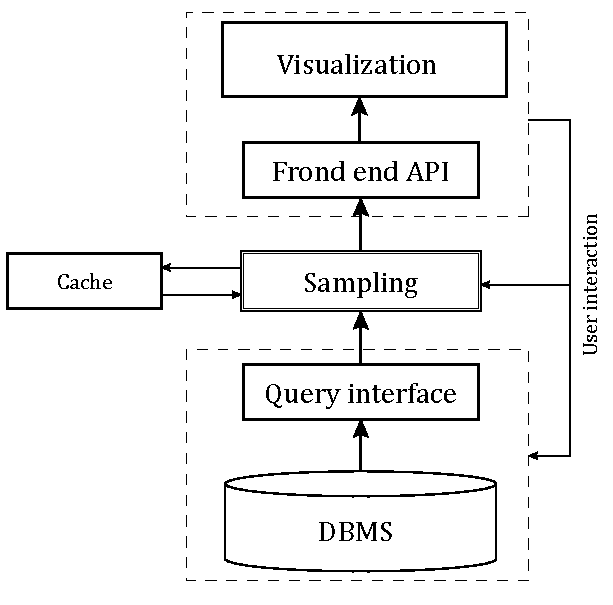
\includegraphics[width=0.3\textwidth]{pictures/framework/DBVAframework.pdf}
	\vspace{-5mm}
	\caption{A visualization framework involving sampling layer between the front-end and database management system.}
	\vspace{-5mm}
	\label{fig:framework}
\end{figure}

